\section{Introduction}
An experimental program focused on search for exotics and the study of rare mesons requires measurements of a broad scope of final states in order to consolidate the possible evidence of a resonance by looking at different decay modes and explore poorly-studied reaction channels \cite{mesonex}.
The characteristics of the detector and the trigger conditions foreseen for the experiment - 11 GeV electron beam scattering on a 5 cm long LH$_2$ target with multiple prongs in the final state - will allow  measurements of many final states simultaneously. While the hadrons will be detected in CLAS12, the electron scattered at very small angles and low four-momentum transfer, $Q^2$,  will be detected in the Forward Tagger (FT), i.e. in the kinematics of quasi-real photoproduction.
The FT  specifications  were thus defined to have the optimal electron detection at low angles compatible with the high rate of electromagnetic background.
To reconstruct the  quasi-real photon variables is necessary to measure the scattered electron three momentum.
The relevant quantities are:
\begin{itemize}
\item the energy E$_{e'}$: since the photon energy is given by E$_\gamma$=$\nu$=E$_{Beam}$-E$_{e'}$ and its linear polarization
 by $P_\gamma=\epsilon^{-1}=1+\frac{\nu^2}{2 E_{Beam} E_{e'}}$,
\item the polar angle $\phi_{e'}$ to determine the polarization plane, 
\item the azimuthal angle angle $\theta_{e'}$: since $Q^2 = 4 E_{Beam} E_{e'} \sin^2{\theta/2}$.
\end{itemize}

The Forward Tagger is composed by: 
an electromagnetic calorimeter  (FT-Cal), to identify the
electron, measure the electromagnetic shower energy and provide a fast trigger signal, a tracker (FT-Trck),  to measure the scattering angles ($\theta_{e'}$ and $\phi_{e'}$) with the required accuracy and a  scintillation counter (FT-Hodo) to provide $e/\gamma$ separation. A dedicated trigger system has been develop to provide a fast signal to trigger the data acquisition in coincidence with signals from CLAS12.
\begin{figure}[th!]
\centering 
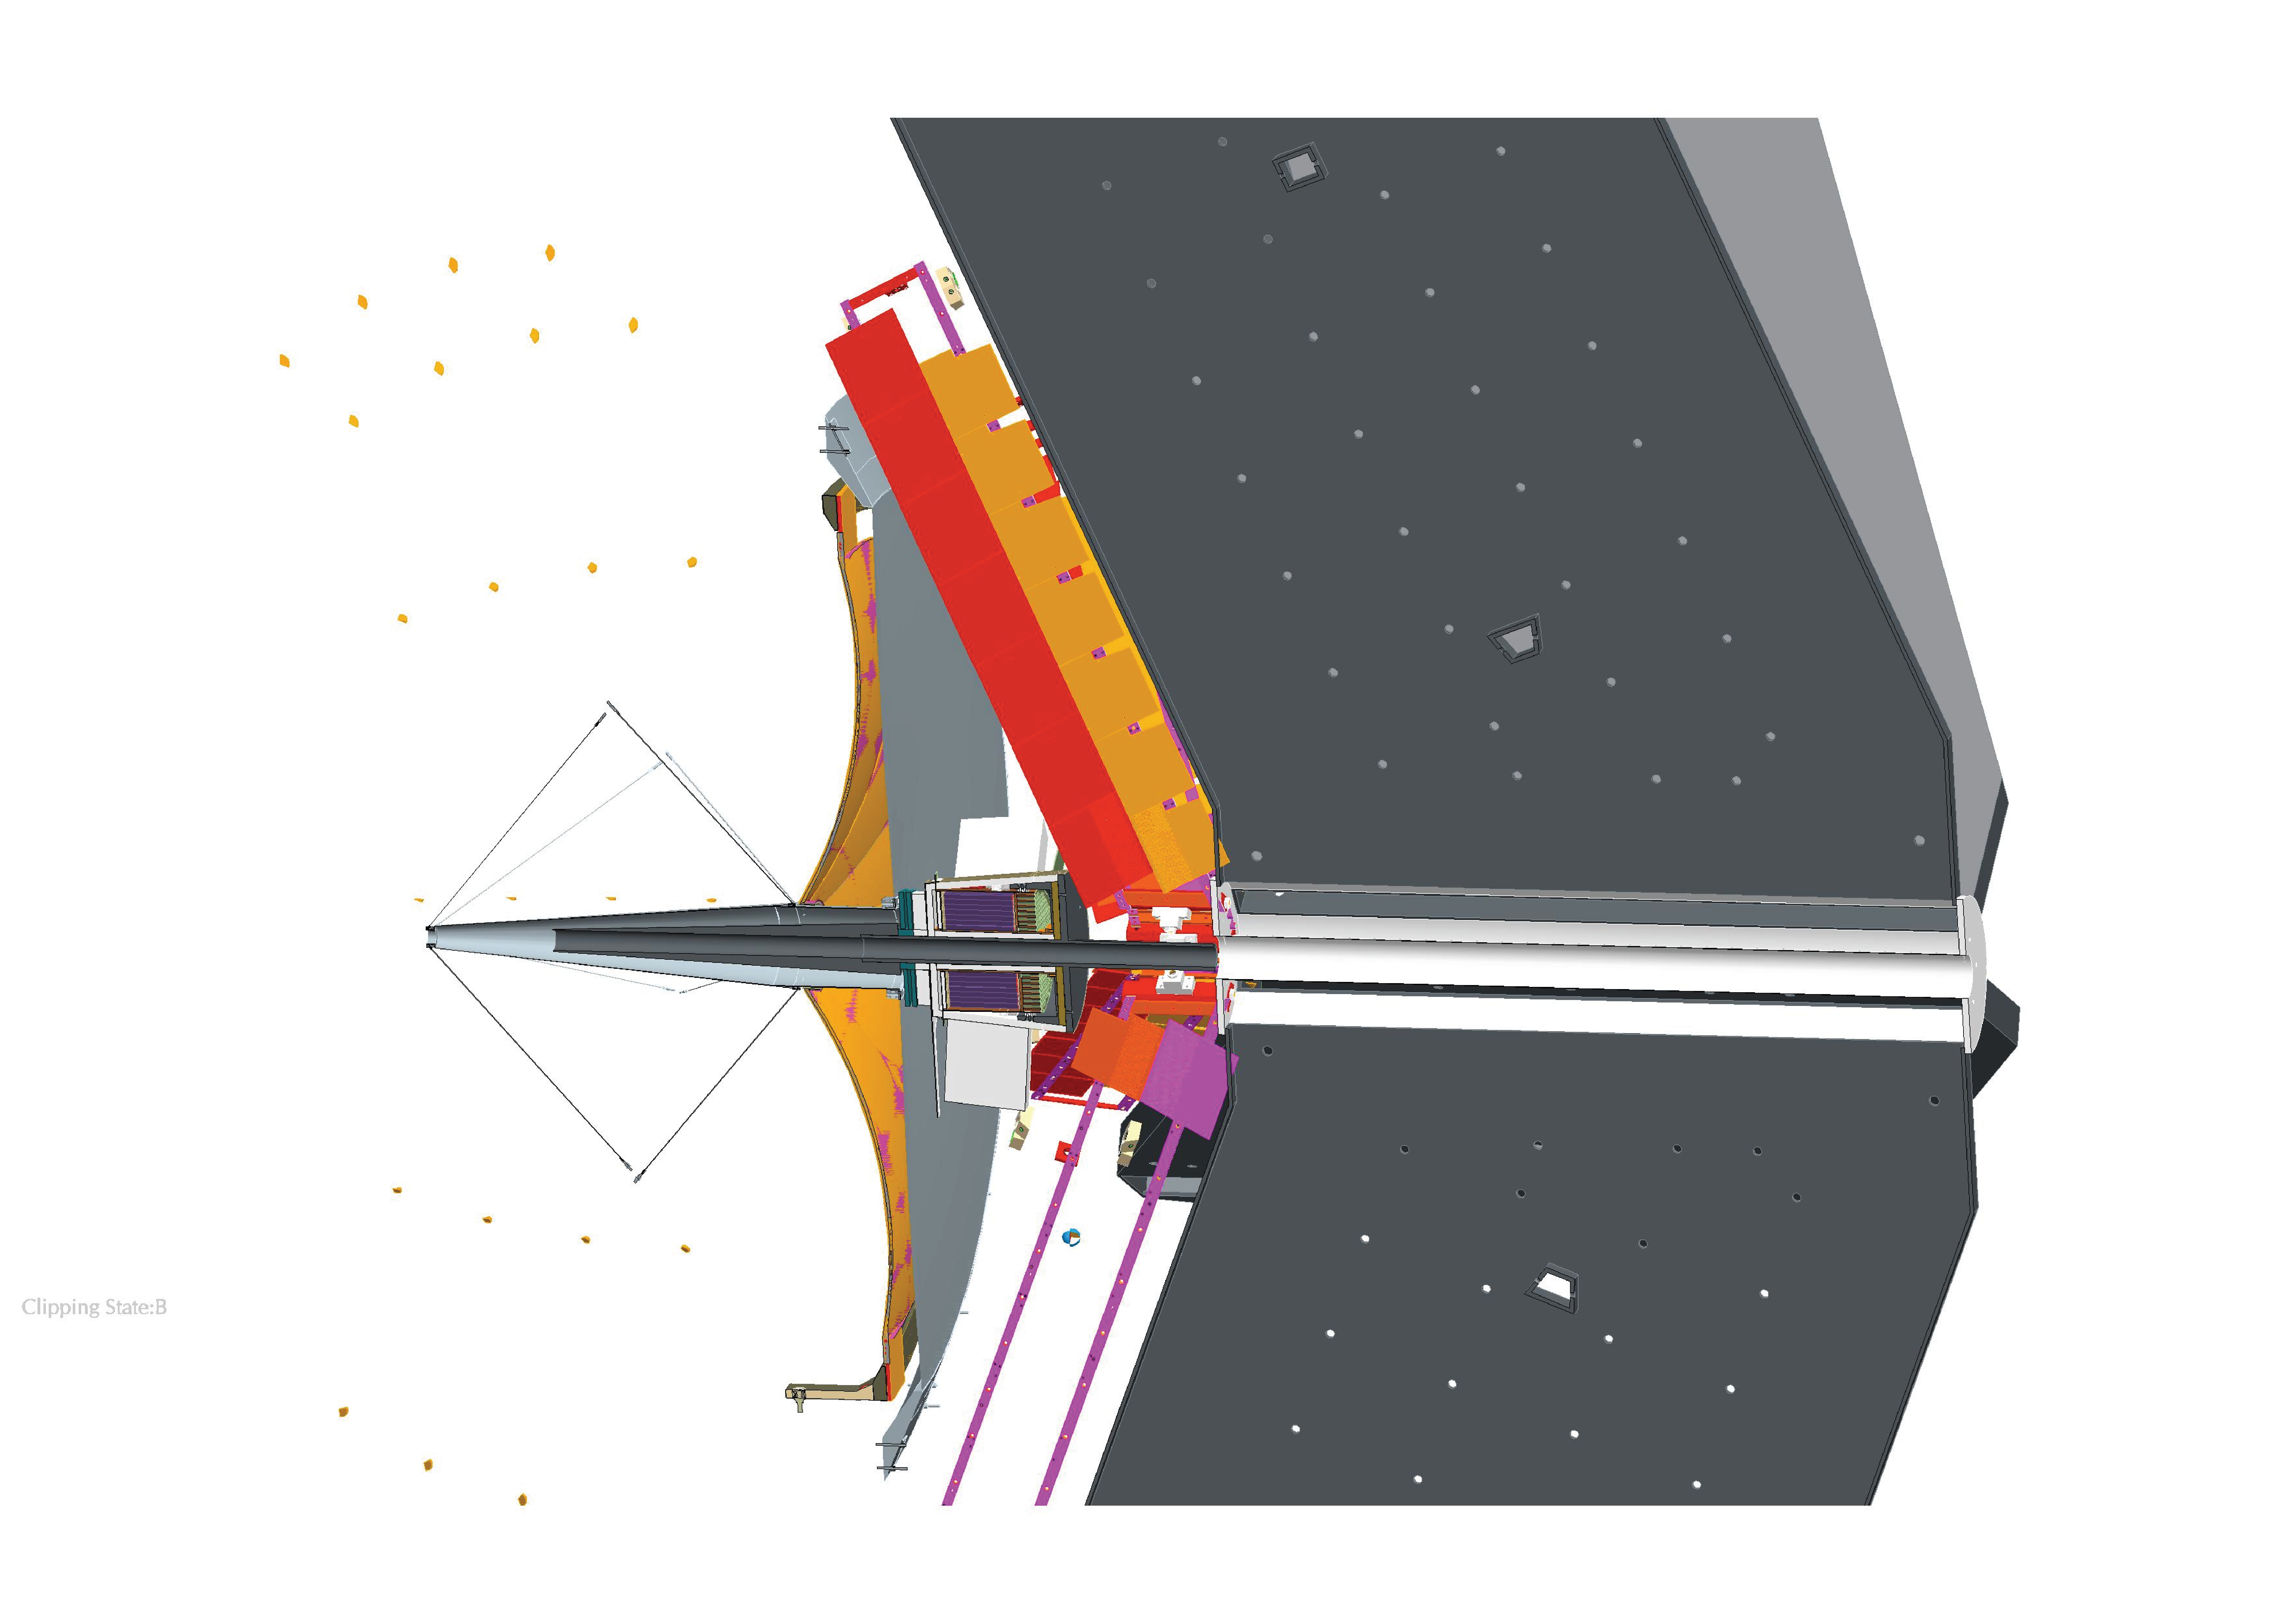
\includegraphics[width=\columnwidth]{./fig/ft_cad.eps} 
\caption{CAD drawing showing the integration of the FT in CLAS12. The FT is located in the free space between the HTCC \cite{htcc} and the first DC layer \cite{dc}. The FT calorimeter shown in blue is located at about 185 cm from the interaction point, shown by the green cross, and is enclosed in a Rohacell case to provide thermal insulation. The scintillation counter (green) and first tracker layer (red) are located in front of the calorimeter. A tungsten cone in black shield the FT from M{\o}ller electrons and electromagnetic background created by the beam. } 
\label{fig:calinclas12} 
\end{figure}

The calorimeter, the scintillation counter and the tracker
are placed between the High Threshold Cerenkov Counter (HTCC)  and the torus support, at about 185 cm downstream of the target (nominal) position. The close proximity
to the beam line ($2.5^\circ$ corresponds to $\sim 8$ cm) and the limited space available (at most $\sim 40$ cm along the beam axis), requires a compact calorimeter with small radiation length and with very good radiation hardness. Figure~\ref{fig:calinclas12} shows 
a CAD drawing of the FT integrated in CLAS12. 
The scintillation counter, placed in front of the calorimeter, is made of plastic scintillator tiles 
read-out by silicon photomultipliers via wavelength shifting fibers. The tracking detector is then located in front of the scintillation counter to extend the CLAS12 forward tracker down to 2.5 degrees.
All these components were designed to fit within a 5.5$^{\circ}$ cone around the beam axis to have no impact on the operation and acceptance of the CLAS12 equipment.
